\documentclass[aps,prb,twocolumn,letterpaper,twoside,nobalancelastpage,groupedaddress,amsmath,amssymb,floatfix,citeautoscript]{revtex4-1}
%\usepackage{geometry}       
%\geometry{letterpaper}     
%\usepackage[parfill]{parskip}    % Activate to begin paragraphs with an empty line rather than an indent
\usepackage{graphicx}
\usepackage{bm} %bold math symbols
\usepackage{times}
\usepackage{graphicx}
\usepackage{physics}
\usepackage{outlines}             
\usepackage{amssymb}
\usepackage[caption=false]{subfig}
\usepackage{mathtools}
\usepackage{color}
\definecolor{darkred}{rgb}{0.6,0.,0.}
\definecolor{darkgreen}{rgb}{0.,0.5,0.}
\definecolor{darkblue}{rgb}{0.,0.,0.6}

\usepackage{framed}

%\usepackage[square,numbers,sort,merge]{natbib}
\usepackage[
breaklinks,
colorlinks=true,
linkcolor=darkred,
citecolor=darkgreen,
urlcolor=darkblue]{hyperref}
%\usepackage{doi}

% \DeclareMathOperator{\tr}{tr}
% \DeclareMathOperator{\erf}{Erf}

\DeclareGraphicsRule{.tif}{png}{.png}{`convert #1 `dirname #1`/`basename #1 .tif`.png}

\begin{document}

\def \Ns {\mathbb{N}}
\def \Rs {\mathbb{R}}
\def \Zs {\mathbb{Z}}
\def \Qs {\mathbb{Q}}
\def \Cs {\mathbb{C}}
\def \id {\mathbb{I}}

\def \bfq {{\bf q}}
\def \bfp {{\bf p}}
\def \bfx {{\bf x}}
\def \bfy {{\bf y}}
\def \bfz {{\bf z}}
\def \bfr {{\bf r}}
\def \bfk {{\bf k}}
\def \bfn {{\bf n}}
\def \bfb {{\bf b}}
\def \bfm {\mathbf{m}}
\def \bfn {\mathbf{n}}

%\def \hata {{a}}
%\def \hatadag {{a}^{\dagger}}

\def \hatq {\widehat{q}}
\def \hatp {\widehat{p}}
\def \hata {\widehat{a}}
\def \hatadag {\widehat{a}^{\dagger}}
%\def \hatb {\widehat{b}^\phantom{\dagger}}
%\def \hatbdag {\widehat{b}^{\dagger}}
\def \wtN {\widetilde{N}}

\def \ve {\varepsilon}
\def \vth {\vartheta}

\title{Non-Landau level cyclotron orbits and the quantum Hall effect in Harper-Hofstadter bands}
\author{David Bauer}
\email{dbauer@physics.ucla.edu}
\affiliation{Department of Physics and Astronomy, University of California at Los Angeles, 475 Portola Plaza, Los Angeles, California 90095, USA}

\author{Fenner Harper}
\affiliation{Department of Physics and Astronomy, University of California at Los Angeles, 475 Portola Plaza, Los Angeles, California 90095, USA}

\author{Rahul Roy}
\affiliation{Department of Physics and Astronomy, University of California at Los Angeles, 475 Portola Plaza, Los Angeles, California 90095, USA}

\date{\today}
\begin{abstract}
Recent developments in fractional quantum Hall (FQH) physics suggest the importance of studying FQH phases of particles occupying single-particle states that are not Landau levels. FQH phases in the regime of strong lattice effects, called fractional Chern insulators (FCI), provide one setting for such studies. As the stength of lattice effects vanishes, the bands of generic lattice models asymptotically approach Landau levels. In this article, we construct non-generic lattice models for single-particle bands that are distinct from Landau levels even in this asymptotic limit. In particular, we study a finely-tuned model with effective continuum hamiltonian with purely quartic dependence on momentum. We describe how the distinction between such bands and Landau levels may be quantified by magnetic Brillouin zone (MBZ) geometry, and we compare the stability of FQH phases in various regimes.
\end{abstract}

% \pacs{0}

\maketitle

\section{Introduction}
The incompressible liquid phases of the fractional quantum Hall effect (FQHE) serve as prototypical examples of topologically ordered or gapped quantum liquid phases\cite{yoshioka_quantum_2002,fradkin_field_2013} in 2+1 dimensions. These phases are characterized by their long-range entanglement structure, which gives rise to topological quasiparticles and universal, quantized linear responses. Theoretical models of the quantum Hall (QH) fluid -- based, for example, on model wavefunctions \cite{laughlin_anomalous_1983} -- often make the simplifying assumption that the microscopic constitutent particles occupy states in a single Landau level. Some properties of Landau levels, such as nonzero Chern number \cite{thouless_quantized_1982}, are essential for the QHE, but recent work points to a need to understand the QHE in the case that the single-particle states are not Landau levels.

Among such work is the observation, due to Haldane, that the FQH fluid carries an emergent geometrical degree of freedom\cite{haldane_geometrical_2011} corresponding to the shape of elementary composite particles or `droplets.' \cite{johri_probing_2016} The geometry of the FQH fluid manifests in part through universal contributions to linear responses corresponding to perturbative variations in geometry, of which the Hall viscosity\cite{avron_viscosity_1995,tokatly_lorentz_2007,read_non-abelian_2009,haldane_hall_2009} is an example. In topological fluids, the Hall viscosity has a universal part proportional to the topological spin of the fluid\cite{read_non-abelian_2009}, which is related to the composite droplet shape.\cite{johri_probing_2016} This geometrical degree of freedom may be obscured by the introduction of non-generic symmetries to the FQH problem implicitly, via the assumption that the underlying single-particle bands are Landau levels.

The study of the FQH beyond Landau levels has also been spurred by the discovery of fractional Chern insulators (FCI) -- time-reversal (TR) symmetry-breaking, fractionalized phases observed in the regime of strong lattice effects \cite{Bergholtz:2013ue,parameswaran_fractional_2013}. In this regime, the single-particle states reside in Chern bands rather than Landau levels. The addition of a non-negligible lattice potential introduces additional geometric data that may break some non-generic symmetries. For example, in the case of a square lattice, $SO(2)$ rotational invariance in the coordinate plane is explicitly broken to $C_4$ lattice symmetry. From this point of view, a complete theory of the FQHE formulated as generically as possible should furnish a theory of FCI phases. Understanding how the lattice potential of FCIs affects the geometrical responses of their topological fluid states is an active research subject. \cite{shapourian_viscoelastic_2015}

 In this article, we study the geometry of Chern bands over the magnetic Brillouin zone (MBZ) parameterizing eigenstates of magnetic translations operators\cite{zak_magnetic_1964}. While this geometry is distinct from the emergent, many-body geometry of the FQH fluid, studies of FCIs have described how single-particle geometry influences the stability of many-body FQH phases through the GMP/$w_{\infty}$ algebra of band-projected density operators.\cite{Girvin:1986bu,parameswaran_fractional_2012,parameswaran_fractional_2013, roy_band_2014} This connection is substantiated by numerical studies \cite{jackson_geometric_2015,Claassen2015,bauer_quantum_2016}, and researchers have employed it to engineer `ideally' stable FCI models \cite{Lee2017}. Chern band geometry can also be understood as the lattice analogue of the continuum, cyclotron-orbit geometry studied in Ref. \onlinecite{haldane_geometry_2015}.

 Experimental signatures of FCIs have been observed in a system of interacting electrons coupled to a superlattice potential generated in a bilayer graphene heterostructure \cite{Spantoneaan8458}. The electrons in the superlattice form Harper-Hofstadter bands with non-zero Chern number. At fractional fillings corresponding to Laughlin states in the conventional FQHE, a gapped phase with fractionally-quantized Hall conductance is observed. \cite{Spantoneaan8458} Other experimental works have identified single-particle Chern bands in the FCI regime. \cite{Jotzu2014,Aidelsburger:2014hm,Aidelsburger:2013ew} Chern bands can be realized in periodically-driven quantum or Floquet systems and their Berry curvature engineered and measured.\cite{Flaschner1091}

Interest in the FQHE in the presence of a lattice potential \cite{kol_fractional_1993,palmer_high-field_2006}..., but FCIs redoubled interest in the subject with the promise of realizing FQH phases outside the usual 2DEG regime. The distinction between FCI models and Harper-Hofstadter \cite{harper_general_1955,Azbel:1964tk,hofstadter_energy_1976} models for lattice electron gasses is nominally that the former have no \textit{net} magnetic field per unit cell, as in the Haldane Chern insulator model\cite{haldane_model_1988}. From a theoretical point of view, this distinction is unecessary \cite{mcgreevy_wave_2012}, and we view FCIs simply as the limit of Harper-Hofstadter models when lattice effects are strong. 

In this article, we discuss Hofstadter-like tight-binding models with additional, longer-range hoppings, in particular focusing on the relationship between the continuum limit of these models and the Landau level hamiltonian. As we will argue in the following section, the bands of such models will generically reproduce Landau levels in the continuum limit. Our main result is to construct such a model that does not have Landau levels as its effective continuum bands. In particular, by adding an additional next-nearest-neighbor hopping term with a negative hopping amplitude, we tune the effective continuum hamiltonian so that the quadratic term vanishes, giving a hamiltonian quartic in momentum to lowest order. This provides a novel setting in which to study quantum Hall systems that is distinct from both the FCI and continuum 2DEG regimes. We focus mainly on a particular choice of hopping amplitudes for the sake of concreteness, but note that different choices of hopping amplitudes lead to an infinite family of non-Landau level continuum bands. We discuss the Chern band geometry of this non-Landau level model, which we use to quantify differences between these bands and Landau levels. We study the stability of the $\nu=1/3$ Laughlin phase by numerical exact diagonalization of a repulsive, many-body hamiltonian projected to the lowest band of this lattice model, and we observe the signatures of the Laughlin phase in the spectrum of the many-body hamiltonian. We focus mainly on the weak-field, effective continuum limit behavior, although some of our numerics should be relevant to fractional Chern insulators.


% We work primarily with the weak-field limit of modified Harper-Hofstadter tight-binding models\cite{harper_general_1955,Azbel:1964tk} on a square lattice. In the presence of spatial inversion symmetry, the weak-field, effective dispersion of Chern bands in these models is generically quadratic, leading to cyclotron degrees of freedom that asymptotically reproduce Landau levels\cite{Harper:2014vi,haldane_geometry_2015}. The main result of our article is the construction of a finely-tuned, tight-binding model with Chern bands that do not approach Landau levels asymptotically in the weak-field limit. That is, we construct a model that is distinct from both FCIs and the Landau level fixed point of weak-field lattice models.

\section{Preliminary Discussion}
\subsection{Landau levels}
\label{landau-level-review}
Since Landau levels serve as our prototype for more general Chern bands, we begin by briefly recalling some physics of Landau levels\cite{yoshioka_quantum_2002}. We study a single electron in two dimensions in the presence of a uniform, perpendicular magnetic field $B$. The single-particle hamiltonian for non-zero $B$ is
\begin{align}
\label{landau-hamiltonian}
H_0 = \frac{1}{2m}\left(\pi_1^2 + \pi_2^2\right),
\end{align}
where $\pi_a = p_a - e A_a(\mathbf{r})$ is the gauge-covariant dynamical momentum and $p_a$ is the gauge-invariant canonical momentum. The operators $H_0$, $\pi_1$ and $\pi_2$ form a three-dimensional Heisenberg Lie algebra $\mathfrak{h}$, with commutators $\comm{H_0}{\pi_1} = \comm{H_0}{\pi_2} = 0$, and $\comm{\pi_1}{\pi_2} = i\hbar^2\ell^{-2}$, where we have introduced the \textit{magnetic length} $\ell = \sqrt{\frac{\hbar}{eB}}.$

% An isomorphic presentation of this algebra is obtained by defining the \textit{cyclotron position operators}
% \begin{align*}
% \mathcal{R}_a = \frac{\ell^2}{\hbar}\epsilon_{ab}\pi_a,
% \end{align*}
% with $\comm{\mathcal{R}_a}{\mathcal{R}_b} = -i\ell^2\epsilon_{ab}$. In terms of these operators, 
% \begin{align*}
% H_0 = \frac{\hbar^2}{2m\ell^4}\left(\mathcal{R}^2_1 + \mathcal{R}^2_2\right),
% \end{align*}
% and we have $\comm{H_0}{\mathcal{R}_1} = \comm{H_0}{\mathcal{R}_2} = 0$.

We then define \textit{guiding-center position operators}
\begin{align*}
R_a = r_a - \frac{\ell^2}{\hbar}\epsilon_{ab}\pi_a,
\end{align*}
which obey commutation relations $\comm{R_a}{R_b} = i\ell^2 \epsilon_{ab}$ and $\comm{R_a}{\pi_b} = 0$, and $\comm{H_0}{R_a} = 0$. We see that the guiding-center and cyclotron operators each form distinct Heisenberg algebras. These algebras have opposite ``handedness,'' in that the commutator $\comm{R_1}{R_2} = i\ell^2$ while $\comm{\mathcal{R}_1}{\mathcal{R}_2} = -i\ell^2$. This decomposition holds in any gauge, although the specific expressions for $\mathcal{R}_a$, $R_a$, and $H_0$ in terms of the gauge-invariant positions and momenta $r_a$, $p_a$ depend on the gauge choice.

We obtain representations of the Heisenberg algebras by a choice of Fock or ladder operators, which are complex linear combinations of the position operators satisfying
\begin{align*}
\comm{a(\boldsymbol{\mathcal{R}})}{a^{\dag}(\boldsymbol{\mathcal{R}})} &= 1, \\
\comm{b(\boldsymbol{R})}{b^{\dag}(\boldsymbol{R})} &= 1.
\end{align*}
This choice is equivalent to a choice of linear complex structure on the respective coordinate spaces. The states 
\begin{align}
\label{basis-state}
\ket{n,m} = \frac{\left(a^{\dag}\right)^n}{\sqrt{n!}}\frac{\left(b^{\dag}\right)^m}{\sqrt{m}} \ket{0,0}.
\end{align}
form a basis for the Hilbert space. For the Landau level hamiltonian (\ref{landau-hamiltonian}), we may choose the cyclotron Fock operators $a$, $a^{\dag}$ such that
\begin{align*}
H_0 = \hbar \omega \left(a^{\dag}a + a a^{\dag}\right).
\end{align*}
Since the hamiltonian is central with respect to both Heisenberg algebras, the basis states $\ket{n,m}$ are eigenstates of $H_0$:
\begin{align*}
H_0 \ket{n,m} = \hbar \omega \left(a^{\dag}a + \frac{1}{2}\right)\ket{n,m}.
\end{align*}
A generic state $\ket{n,\Psi}$ within the $n$th Landau level can be written as a function purely of the $b^{\dag}$ operators applied to the vaccuum state:
\begin{align*}
\ket{n,\Psi} = \Psi(b^{\dag})\ket{n,0}.
\end{align*}

\subsection{Effective Landau levels from weak-field Harper-Hofstadter models}
\label{landau-level-limit}
In this section, we consider the weak-field limit $\phi \rightarrow 0$ of a Harper-Hofstadter tight-binding hamiltonian, and show that to lowest order in $\phi$, this hamiltonian reproduces the Landau level hamiltonian

We introduce a uniform background magnetic field $B$ perpendicular to the spatial extent of the lattice. We choose the value of $B$ to be such that the flux per lattice plaquette is $\phi = Ba^2 = \frac{P}{Q}\phi_0$, where $\phi_0 = 2\pi \hbar /e$ is the magnetic flux quantum and $P$ and $Q$ are relatively prime integers. We will mostly have in mind the case $P =1$, in which the band structure is on conceptually simplest.\cite{Harper:2014vi} In terms of the magnetic length and lattice spacing, $\phi = \frac{\hbar}{e}\frac{a^2}{\ell^2}$. For the rest of this article, we will work in units in which $\frac{\hbar}{e}= 1$, so that $\phi =\frac{a^2}{\ell^2}$ is a dimensionless ratio of length scales.

In the presence of the magnetic field, the naive translation operators are not gauge invariant \cite{fradkin_field_2013}, and we must accompany translations by compensatory gauge transformations. The gauge invariant translation operators are
\begin{align*}
T_a = \sum_{\mathbf{m}} e^{i\theta_a(\mathbf{m})} c^{\dag}_{\mathbf{m} + \mathbf{e}_a}c_{\mathbf{m}}.
\end{align*}
where the phases $e^{i\theta_a(\bfm)}$ satisfy 
\begin{align*}
\theta_1(\bfm) + \theta_2(\bfm + \mathbf{e}_1) - \theta_1(\bfm + \mathbf{e}_2) - \theta_2(\bfm) = \phi,
\end{align*}
% or
% \begin{align*}
% \Delta_1\theta_2 - \Delta_2\theta_1 = \varepsilon^2.
% \end{align*}
We regard the phases $\theta$ as residing on the links of the lattice, but we canonically identify $\theta_a(\mathbf{m}) = \theta(\mathbf{m},\mathbf{m}+\mathbf{e}_a)$. The components of $\widetilde{\mathbf{T}}$ do not commute, but satisfy 
\begin{align*}
T_x T_y = \exp(i\phi^2) T_y T_x.
\end{align*}
The lattice translation operators $T_a$ are unitary, so we can write them in terms of hermitian generators $T_a = \exp\left[i K_a\right]$. The $K_a$ are the lattice analogues of the covariant momentum operators $\pi_a$, and we will sometimes call them mometa for brevity.

%  This implies the commutator
% $\comm{K_x}{K_y} = i \varepsilon^2.$

% Because the $T_a$ do not commute with each other, there is an ambiguity in passing from the $B=0$ hamiltonian to one for $B\neq0$, which appears as a choice of phase of the (now-complex) $t_{\mathbf{m}\mathbf{n}}$. This is analogous to the ordering ambiguity in quantizing polynomials on classical phase space. For now we fix this ambiguity by making the arbitrary choice that $T_x^j T_y^k \rightarrow T_x^j T_y^k + T_y^kT_x^j$ in the presence of nonzero $B$. We could also have fixed this ambiguity by a choice of gauge for the $\theta(\mathbf{m})$. Then
The most general tight-binding hamiltonian we can write down has non-zero hopping amplitudes between any two sites of the lattice. There is an ambiguity constructing such a hamiltonian, because 
\begin{align*}
H_{\text{TB}} = -\sum_{j,k} t_{jk}\left(T_x^j T_y^k + T_y^kT_x^j\right) + \text{h.c.}
\end{align*}
We note that in our convention, the hopping amplitudes $t_{jk}$ are always real, and any complex phase factors come from the action of the translation operators.

Let us look at just the nearest-neighbor (NN) hopping hamiltonian containing only first powers of the translation operators,
\begin{align*}
H_{\text{NN}} = -t_{10}\left(T_x + T_x^{\dag}\right) - t_{01}\left(T_y + T_y^{\dag}\right)
\end{align*}
  % This part of the hamiltonian requires no ordering prescription or gauge choice.
In the $C_4$ symmetric case, $t_{01} = t_{10}$, $H_{\text{NN}}$ is just the hamiltonian of the usual Hofstadter model with non-zero amplitude only for NN hoppings. Since $T_a = e^{iK_a}$,
\begin{align*}
H_{\text{NN}}= -2t_{10}\cos\left(K_x\right) - 2 t_{01}\cos\left(K_y\right).
\end{align*}
In order to make the dependence on $\phi$ explicit, we rescale the $K_a$ operators, defining $\sqrt{\phi} P_a = K_a$. 
\begin{align*}
H_{\text{NN}} &= -2\sum_{n=0}^{\infty}  \frac{(-1)^{n}\phi^{n}}{(2n)!} \left(t_{10} P^{2n}_x + t_{01}P^{2n}_y\right)\\
&= -2 + 2\phi\frac{\left(t P^{2}_x + t' P^{2}_y\right)}{2} +O(\phi^2).
\end{align*}
Now let $t' = \alpha^2 t$, i.e., $t$ is a common hopping energy scale and $\alpha$ parameterizes anisotropy in the hopping amplitudes. Then to lowest order in $\phi$, we have a small-$\phi$ effective hamiltonian $H_{\text{eff}}= t\phi \left(P^{2}_x + \alpha^2P^{2}_y\right)$. We can rewrite this in terms of momentum operators that satisfy $\comm{\pi_x}{\pi_y} = i\hbar e B$ as
\begin{align*}
H_{\text{eff}} = \frac{1}{2m_{\ast}}\left(\pi_x^2 + \pi_y^2\right),
\end{align*}
showing that our effective hamiltonian is isomorphic to the Landau level hamiltonian with effective mass $m_{\ast} = \hbar^2/(2ta^2\alpha)$. In order to recover all of the physics of Landau levels, we also need an analogue of the guiding-center operators that commute with the hamiltonian but not one another, producing an extensive degeneracy. Here, this role is filled by the magnetic translation operators, which we define in the following section. If we consider not just nearest-neighbor but also longer range hopping terms, the details of the above argument are slightly more complicated, but to lowest order the hamiltonian is quadratic in the momenta. This gives us an effective mean-field hamiltonian for the cyclotron degrees of freedom. 

\subsection{Chern bands}
The simulatenous eigenstates of the hamiltonian and MUC translations are $\ket{n,\bfk}$, where $\bfk$ takes values in the magnetic Brillouin zone and $n$ labels eigenstates of $H$. We can write the hamiltonian 
\begin{align}
\label{band-projector-ham}
H = \sum_{n}\int d^2k\, E_{n}(\bfk) P_{n,\bfk},
\end{align}
where $E_n$ is the dispersion of the $n$-th band of the hamiltonian, and $P_{n,\bfk}$ is the projector onto the state $\ket{n,\bfk}$.

Unlike in Landau levels, the dispersion $E_{n}(\bfk)$ generically has some finite width, and the states in the band are not exactly degenerate. In the weak-field case this bandwidth will be exponentially small\cite{Harper:2014vi}, while in the strong-field limit we may follow the usual procedure of adding long-range hoppings to flatten the band. \cite{Bergholtz:2013ue,parameswaran_fractional_2013} In either case, we will neglect the bandwidth. Despite being dispersionless, these Chern bands are distinct from Landau levels. We can quantify this distinction by considering the Berry curvature and Fubini-Study (FS) metric defined on the magnetic Brillouin zone\cite{parameswaran_fractional_2013,roy_band_2014,Claassen2015}. (The FS metric has also been called the Bures metric in this context.\cite{palumbo_momentum-space_2017}) For notational simplicity, we define $\partial_a \coloneqq \partial_{k_a}$. Then, respectively, the Berry curvature and FS metric components for a band with projector $P_{\mathbf{k}}$ are
\begin{align*}
B(\bfk) = \epsilon_{ab}\text{Tr}\left(\partial_{a}P_{\mathbf{k}}\partial_b P_{\mathbf{k}}\right),
\end{align*}
and, defining the orthogonal projector $Q_{\mathbf{k}} = \mathbf{1} - P_{\mathbf{k}}$,
\begin{align*}
g_{ab}(\bfk) = \frac{1}{2}\text{Tr}\left(\partial_{a}Q_{\mathbf{k}}\partial_{b}P_{\mathbf{k}} + \partial_{b}Q_{\mathbf{k}}\partial_{a} P_{\mathbf{k}}\right). \\
%\left. \quad\quad-P_{n,\bfk}\left[\partial_aP_{n,\bfk}\partial_b+ \partial_bP_{n,\bfk}\partial_a\right] P_{n,\bfk}\right)
\end{align*}
The traces in these expressions are taken over the cyclotron Hilbert space. The TR-symmetry breaking Chern bands that we want to study are those with nonvanishing first Chern number 
\begin{align*}
c_1 = \int d^2k\, B(\mathbf{k}).
\end{align*}

\begin{figure}[thb]
\centering
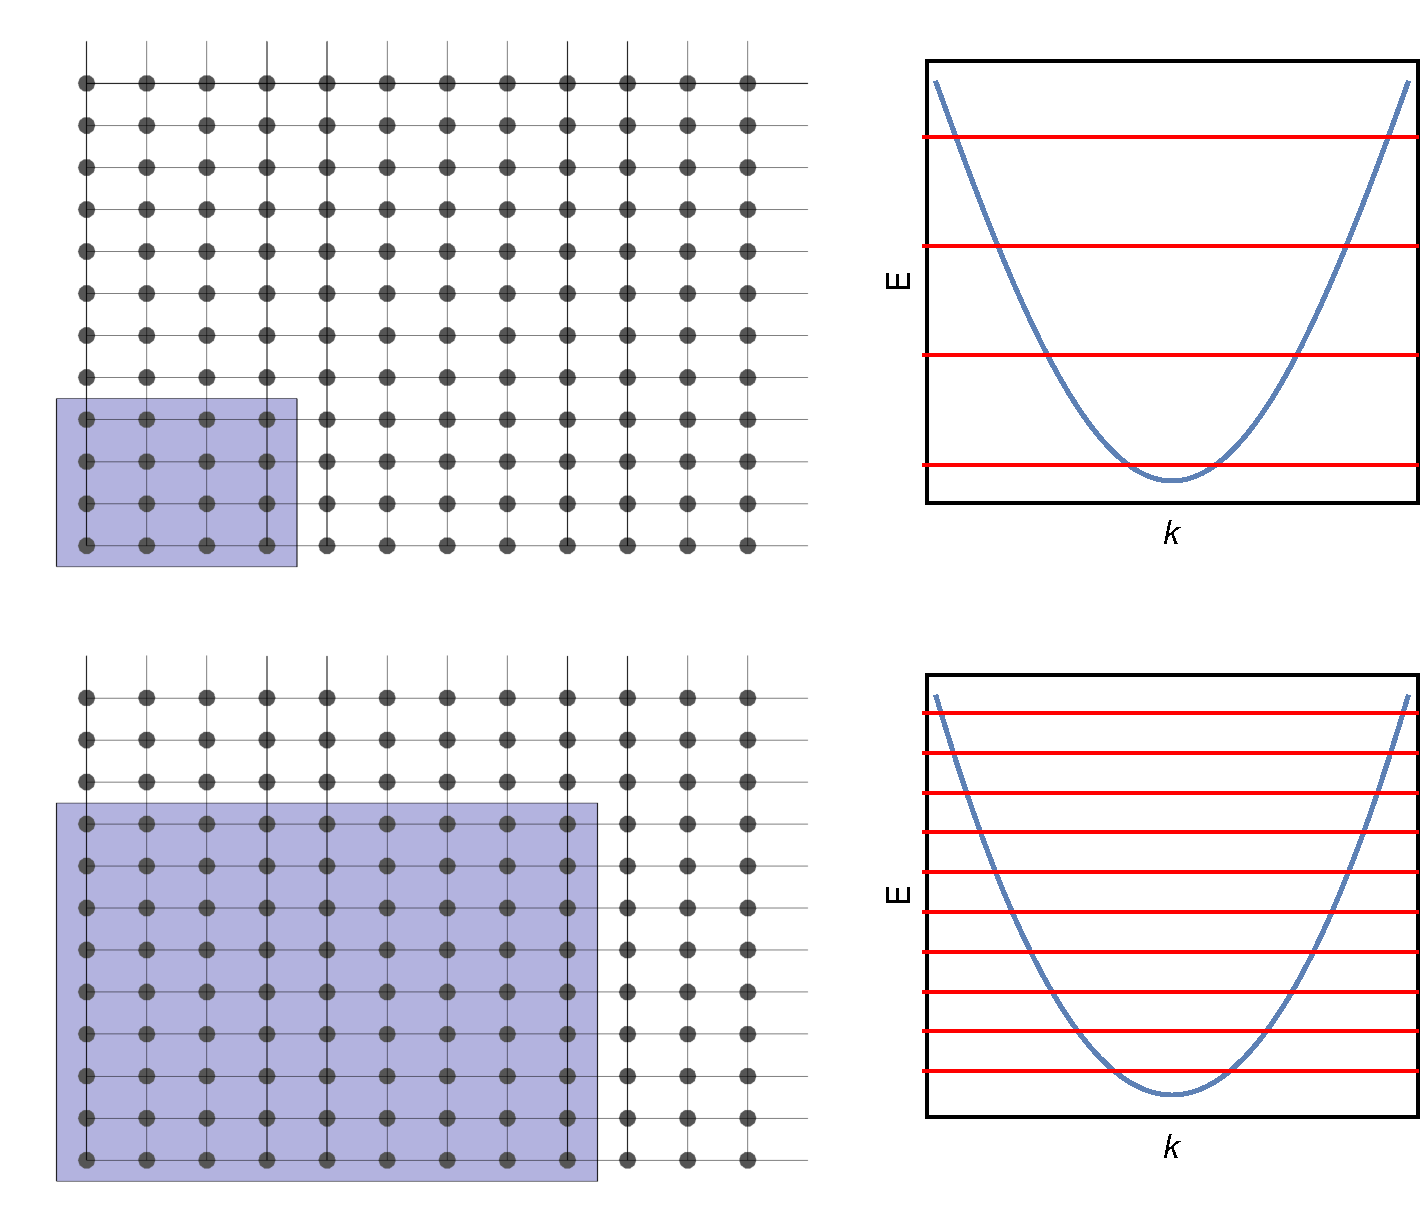
\includegraphics[width=3.1in]{unit-cell-dispersion-grid.pdf}
\caption{\label{bands-schematic}Schematic depiction of Landau-levels as the weak-field limit of Harper-Hofstadter bands near the minimum of a periodic potential. As the flux per plaquette is decreased, the elementary magnetic unit cell -- represented by the blue region of the lattice -- must increase in size to enclose the same number of flux quanta. In turn, the number of states in within each band decreases, and each band comprises states increasingly close to the minimum of the zero-field dispersion.}
\end{figure}

The weak-field/continuum limit is implemented in the $\bfk$-representation by expanding the band dispersion $E_{n}(\bfk)$ near a band minimum. The lowest-order term in such an expansion will generically be quadratic in $\bfk$, which essentially follows from our argument in the previous section. Since the mean electron density $\rho_0$ in QH systems is pegged to the magnetic flux density by the filling fraction
\begin{align*}
\nu = \frac{N_p}{N_s} = N_p\frac{A_{\text{tot}}}{A_{\text{MUC}}}
\end{align*}
the weak-field limit corresponds to the limit of dilute electrons. This leads to a more conceptual picture, shown in cartoon form in Fig. \ref{bands-schematic} for how decreasing flux per plaquette leads to continuum limit Landau levels. If we fix the overall system size and the magnetic flux attached to each guiding-center lattice site (the flux through each MUC), decreasing flux per plaquette must increase the area of each MUC. We therefore increase the number of states in the cyclotron Hilbert space, while decreasing the number of guiding-center states available within each band. The states that live near the band minimum when there is no magnetic field then redistribute into increasingly higher bands as $\phi$ decreases.


\section{Non-Landau effective hamiltonians}
In this section, we introduce and study a new class of weak-field effective hamiltonians that cannot be transformed into the Landau hamiltonian at lowest order in $\phi$. To start, we consider an example of such a hamiltonian that contains only quartic powers of the momenta $K_a$,
\begin{align}
\label{quartic-harper}
H_{\text{TB}} = &-t_1 \left(T_x + T_x^{\dag} + T_y + T_y^{\dag}\right)\nonumber\\ &- t_2 \left(T_x^{2} + T_x^{\dag 2} + T_y^{2} + T_y^{\dag 2}\right).
\end{align}
Note that this hamiltonian only contains straight-line lattice translations, and omits NNN hopping between opposite plaquette corners. Unless explicitly stated, we will assume from here onward that $t_1$ sets the overall scale of the hamiltonian, and set $t_1=1$; the remaining hopping amplitudes in each expression should then be understood as dimensionless ratios.

As in Section \ref{landau-level-limit}, we write this in terms of the hermitian generators of lattice translations,
\begin{align*}
H_{\text{TB}} = &-2\left(\cos(K_x) + \cos(K_y)\right)\\ &- 2t_2\left(\cos(2K_x) + \cos(2K_y)\right)
\end{align*}
Replacing the cosine terms by their Taylor expansion, the terms lowest-order in the momenta are 
\begin{align*}
H_{\text{TB}} = &-4 - 4 t_2 + (1 + 4t_2) \left(K_x^2 + K_y^2\right) \\
&- \left(\frac{1}{12} + \frac{4}{3}t_2\right) \left(K_x^4 + K_y^4\right) + \ldots
\end{align*}

If we make the particular choice of hopping amplitudes $t_2 = -1/4$, then the quadratic terms vanish exactly, and we are left with an effective hamiltonian that is quartic in the momenta to lowest order,
\begin{align}
\label{hamiltonian-quartic-effective}
H_{\text{eff}} = -3 + \frac{1}{4} \left(K_x^4 + K_y^4\right).
\end{align}
Such negative hopping amplitudes can be realized in optical lattice experiments by periodic shaking of the lattice\cite{eckardt_colloquium_2017}. Unlike the Landau level hamiltonian, this hamiltonian does not have $SO(2)$ rotational symmetry, but it is symmetric under the square lattice isometry group $D_4$. 

By introducing additional hopping amplitudes between non-neighboring sites and tuning the amplitudes appropriately, we may eliminate increasingly higher-order terms in the hamiltonian. We focus on the case in which we add only straight-line hoppings, as we did for the quartic model above. For example, we obtain the effective hamiltonian
\begin{align*}
H_{\text{eff}} = K_x^6 + K_y^6
\end{align*}
by choosing $t_{20}=t_{02}=-2/5$ and $t_{30}=t_{03}=1/15$. We can generalize to the case
\begin{align*}
H^{(2n)}_{\text{eff}} = K_x^{2n} + K_y^{2n}
\end{align*}
As we did for the quartic case, we find the  perturbative, finite-size eigenstates numerically and calculate their trace inequality. Interestingly, we find that the trace inequality is maximum for $2n=6$ and that it decreases monotonically at least until $2n=30$.
\begin{figure}[thb]
\centering
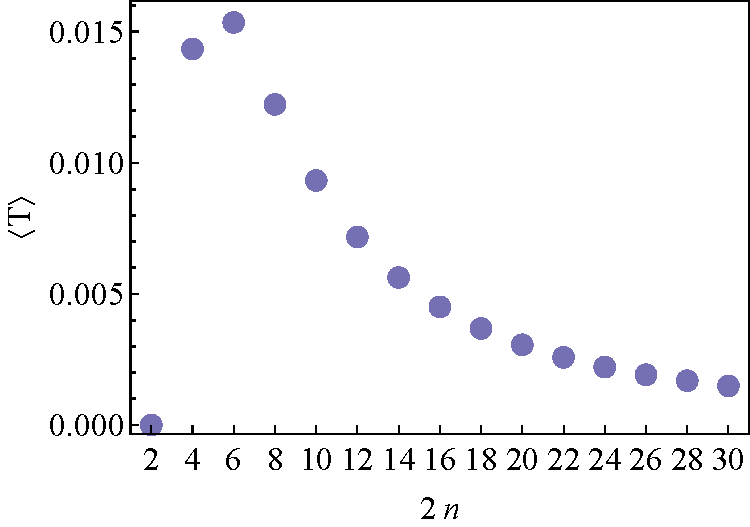
\includegraphics[width=3.0in]{tr-v-2n.pdf}
\caption{Trace inequality $\expval{T} = 2 \expval{a^{\dag} a}$ for the ground state band of the hamiltonian $H^{(2n)}$}
\end{figure}

\subsection{Non-perturbative corrections}
In our perturbative approach to this problem, we expand about a band minimum to obtain an effective mean-field hamiltonian. In doing so, we neglect non-perturbative corrections due to the lattice. However, these corrections decay exponentially in $1/\phi$, as we will now argue.

Intuitively, the exponential dependence on $1/\phi$ follows because the non-perturbative corrections arise from tunneling between band minima. This intuition holds true for the Hofstadter model, for which non-perturbative fluctuations in the dispersion and Berry curvature and the Fubini-Study metric decay exponentially in $1/\phi$. 

In our case, the situation is not much different, because WKB approximation employed in studying the Hofstadter model is not sensitive to the order of the differential (or difference) equation. That is, we may use the WKB ansatz
\begin{align}
\label{wkb-ansatz}
\psi(x) = \exp\left[\frac{1}{\phi}\left(S_0(x) + \phi S_1(x)\right)\right],
\end{align}
for any Harper-type equation
\begin{align*}
\sum_{n}\phi^{2n}\Delta^{(2n)}\psi(x) = \left[-\epsilon - V(x)\right]\psi(x).
\end{align*}
with the same constraints on the region of validty that apply to the usual Harper equation. We have introduced the $2n$-th central finite difference operator $\Delta^{(2n)}$ here. Employing this ansatz in the classically-forbidden or tunnelling region, this ansatz yields
\begin{align}
\label{wkb-solution}
\psi(x) = \exp\left[\frac{1}{\phi}\left(S_0(x) + \phi S_1(x)\right)\right],
\end{align}

\begin{figure}[thb]
\centering
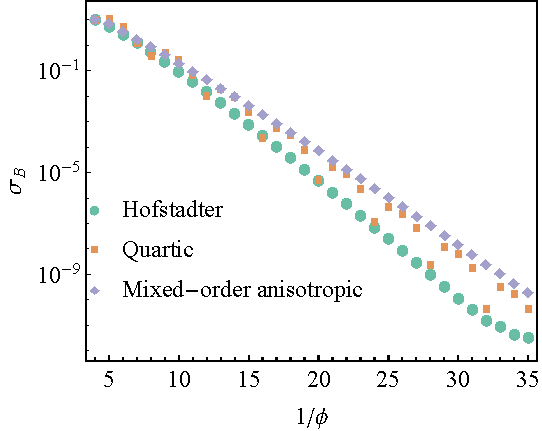
\includegraphics[width=3.0in]{rms-curv-fluct.pdf}
\caption{RMS fluctuation $\sigma_B$ of Berry curvature $B$ from its average value on the MBZ.}
\end{figure}

\subsection{Example: Quartic model}
We now return to consider some details of the model given by Eq. (\ref{hamiltonian-quartic-effective}), in particular its continuum limit. We plot the energy eigenvalues obtained from the Harper-type equation for this model as a function of $\phi$ -- the analogue of the Hofstadter ``butterfly'' for this model\cite{hofstadter_energy_1976}. We display this in Fig. \ref{butterfly-plot}. In the Hofstadter model, where the bands appear approximately linear in $\phi$ near $\phi = 0$, the present model has bands that are roughly quadratic in $\phi$ in this region. We compute the Berry curvature and Chern number of these bands for $\phi = \frac{1}{N}$ and verify that they have Chern number $|c_1| = 1$.

\begin{figure}[thb]
\centering
\hspace{-0.25in}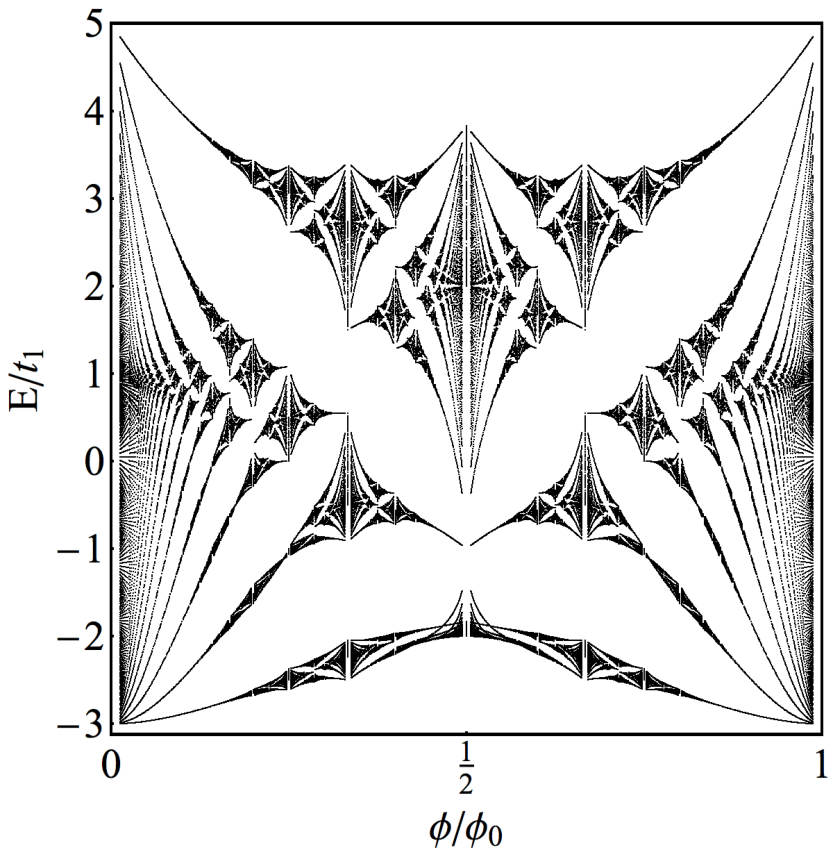
\includegraphics[width=3.0in]{q-butterfly-raster-1200.pdf}
\caption{\label{butterfly-plot} Energy eigenvalues of the lattice Harper-Hofstadter hamiltonian (\ref{quartic-harper}) with $t_1 = 1$, $t_2 = -1/4$ as a function of magnetic flux per elementary lattice plaquette $\phi = P/Q$.}
\end{figure}

% \begin{figure}[thb]
% \centering
% 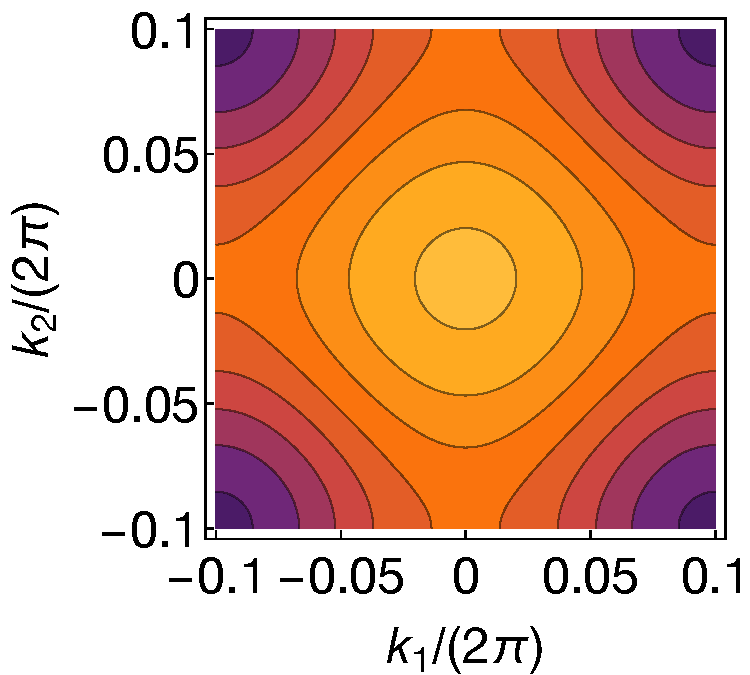
\includegraphics[width=1.4in]{curv-hof-n5.pdf}
% 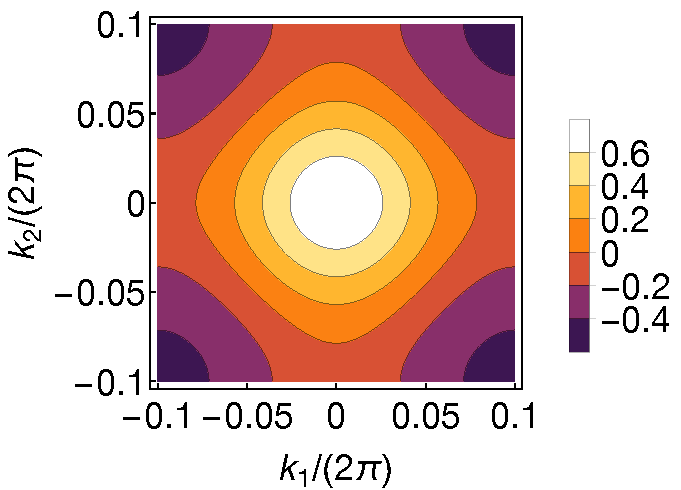
\includegraphics[width=1.75in]{curv-qrt-n5.pdf}
% 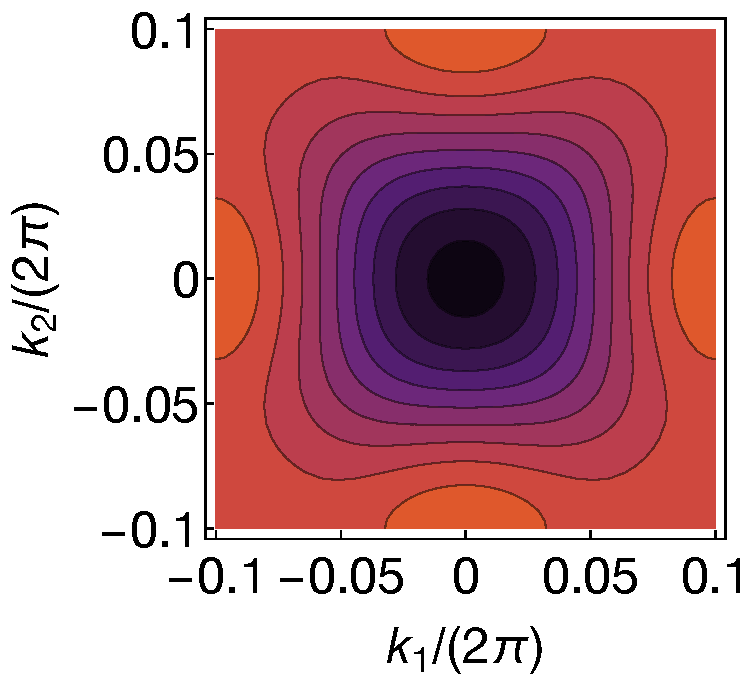
\includegraphics[width=1.4in]{norm-tr-hof-n5.pdf}
% 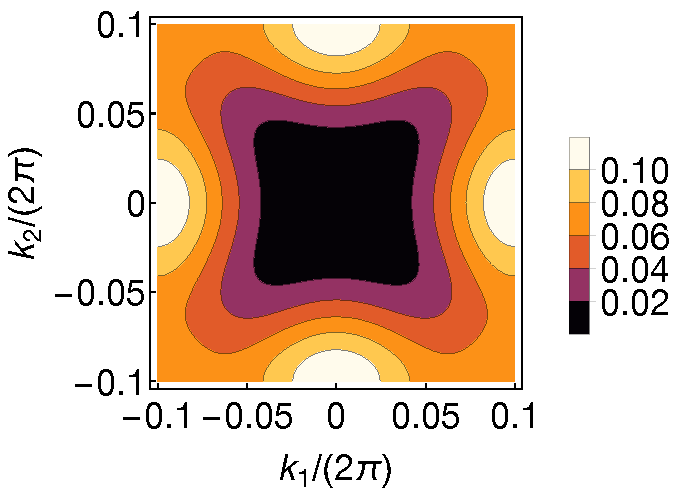
\includegraphics[width=1.75in]{norm-tr-qrt-n5.pdf}
% \caption{Comparison of magnetic Brillouin zone geometry between Hofstadter (left) and quartic (right) models at flux per plaquette $\phi/\phi_0=1/5$. The top left panel shows the Berry curavture $B(\mathbf{k})$ for the Hofstadter model; the top right panel shows $B(\mathbf{k})$ for the quartic model. The bottom panels show the normalized trace inequality $\bar{T}(\mathbf{k})$ for these models.}
% \end{figure}

The particular quartic momentum operator in (\ref{hamiltonian-quartic-effective}) can be written
\begin{align*}
K_x^4 + K_y^4 = \left(K_x^2 + K_y^2\right)^2 - \left(K_x^2K_y^2 + K_y^2K_x^2\right),
\end{align*}
that is, as the square of the Landau-level hamiltonian plus a term that explicitly breaks the rotational symmetry.

As in the Landau level problem, we study the spectrum of this model by introducing ladder operators $a$, $a^{\dag}$ corresponding to the cyclotron momenta $K_a$. For example, we choose the operators
\begin{align*}
a &= \frac{1}{\sqrt{2\phi}}\left(K_x - iK_y\right),\\
a^{\dag} &= \frac{1}{\sqrt{2\phi}}\left(K_x + iK_y\right),
\end{align*}
with inverse map
\begin{align*}
K_x &= \sqrt{\frac{\phi}{2}}\left(a + a^{\dag}\right),\\
K_y &= -i\sqrt{\frac{\phi}{2}}\left(a - a^{\dag}\right).
\end{align*}
We also define the dimensionless operator
\begin{align*}
h_0 = \left(a^{\dag}a + \frac{1}{2}\right).
\end{align*}
In terms of these operators,
\begin{align*}
\left(K_x^2 + K_y^2\right)^2 &= \phi^2\left(4 h_0^2\right), \\
\left(K_x^2K_y^2 + K_y^2K_x^2\right) &= \phi^2\left(h_0^2 -\frac{1}{2}\left(a^4 + a^{\dag\,4}\right) - \frac{3}{4}\right),
\end{align*}
and the effective hamiltonian is
\begin{align}
\label{effective-fock-hamiltonian}
H_{\text{eff}} = \frac{\phi^2}{8}\left[\left(a^4 + a^{\dag 4}\right) + 6h_0^2 + \frac{3}{2}\right].
\end{align}

We numerically approximate this hamiltonian by working in a basis of number eiegenstates $\ket{n}$ staisfying $a^{\dag}a{\ket{n}}=n{\ket{n}}$ and truncating to a finite-dimensional subspace. This gives estimates for the cyclotron energies and overlaps with the Landau level states. We find good agreement between this continuum approximation truncated to $n \leq 1000$ and exact numerical energy levels of lattice hamiltonian for small $\varepsilon$. The first two nonzero overlaps of the ground state $\ket{\tilde{0}}$ of the hamiltonian (\ref{effective-fock-hamiltonian}) with the Landau level states are $\braket{\tilde{0}}{0}\approx0.9991$, $\braket{\tilde{0}}{4}\approx-0.0422$. When expressed with ladder operators, the trace inequality takes the particularly simple form $\expval{T} = 2\expval{a^{\dag}a}$\cite{bauer_quantum_2016}; that is, $\expval{T}$ is twice the mean LL occupation number $n_0$. Calculating this in the truncated Landau level basis, we find $\expval{T} \approx0.0143$, in good agreement with the value found from intergrating the lattice $T(\mathbf{k})$ over the MBZ, $\expval{T} \approx 0.0145$.

We also study the spectrum of cyclotron orbits of this hamiltonian semiclassically by applying the Bohr-Sommerfeld quantization condition that the adiabatic invariants of the classical hamiltonian be quantized. In our notation, this condition takes the form
\begin{align*}
\oint\limits_{H=E_n} K_x\, dK_y = 2\pi n,
\end{align*}
with the integral taken over a closed curve of constant energy in classical phase space. From this condition we find
\begin{align*}
E_n \sim n^2\phi^2, 
\end{align*}
in agreement both with the numerically-obtained, approximate spacing of the cyclotron levels, and with the quadratic dependence of $E$ on $\phi$ observed in the butterfly plot, Fig. \ref{butterfly-plot}.

We now consider general values of $t_2$. The effective hamiltonian is
\begin{align}
\label{t2-hamiltonian}
H_{\text{eff}} = &-\frac{1 + 16t_2}{12}\left(K_x^4 + K_y^4\right)\nonumber\\ &+ \left(1 + 4t_2\right) \left(K_x^2 + K_y^2\right),
\end{align}
or
\begin{align*}
H_{\text{eff}} = 2&\phi\left(1 + 4t_2\right) h_0\\  - &\phi^2\frac{\left(1 + 16t_2\right)}{4} \left(h_0^2 + \frac{\left(a^{4} + a^{\dag 4}\right)}{6} + \frac{1}{4}\right)
\end{align*}
For any value of $t_2$ away from the fine-tuned point $t_2 = -1/4$, we may always choose $\phi$ small enough that the quadratic term dominates and we recover the Landau level hamiltonian. However, if we consider $\phi$ small but fixed, we can make the weight of the quadratic term small by tuning $t_2$ appropriately. In this regime, we can treat the quadratic term in the hamiltonian as a perturbation to the quartic term, with perturbative parameter
\begin{align*}
\varepsilon = \frac{8}{\phi}\frac{\left(1 + 4t_2\right)}{\left(1 + 16t_2\right)}.
\end{align*}
A weak upper bound on the regime in which may treat the quadratic term as a perturbation is given by setting $\varepsilon < 1$ or
\begin{align*}
t_2 > -\frac{1}{4} - \frac{3}{32}\phi +O(\phi^2).
\end{align*}


\begin{figure}[thb]
\centering
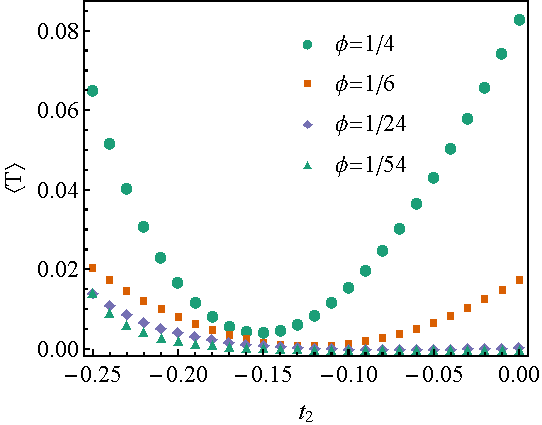
\includegraphics[width=3.0in]{trace-delta-plot-new.pdf}
\caption{\label{trace-delta-plot}Magnetic Brillouin zone-averaged trace inequality $\expval{T}$ for the lowest-lying band of (\ref{quartic-harper}) as a function of $t_2$ with $t_1 = 1$. $t_2 = 0$ is the Hofstadter model, and $t_2 = -1/4$ is the fine-tuned quartic model.}
\end{figure}
\begin{align*}
\end{align*}

\subsection{Hamiltonians with no $h_0$ term}
That the overlap of the groundstate of the quartic model with the LLL is large not surprising, given the large weight of the Landau hamiltonian $h_0$ in (\ref{hamiltonian-quartic-effective}). We might ask whether it is possible eliminate this term entirely, and what impact this has on the spectrum. In fact, we can isolate the $a^4 + a^{\dag 4}$ term by choosing
\begin{align*}
t_{01} = t_{10} = t_1\\
t_{02} = t_{20} = \frac{t_1}{8} \\
t_{11} = - \frac{3}{4}t_1, 
\end{align*}
which gives
\begin{align*}
H_{\text{eff}} = \frac{3}{2} + \frac{\phi^2}{4}(a^4 + a^{\dag\,4})
\end{align*}

This case is distinct from the cases we have considered so far because we are expanding about a local maximum instead of a minimum in the dispersion. The spectrum of this hamiltonian is not bounded from below, so we cannot find its ground states. However, there is a set of degenerate zero-energy states. While we were unable to obtain an analytical form for the coefficients in the LL basis for the ground state of (\ref{hamiltonian-quartic-effective}), that fact that the states here have exactly zero energy makes the current problem tractable. We present an analytical calculation of one of the zero-energy states 

\subsection{Anisotropic models}
In the foregoing, we considered only models invariant under $C_4$ symmetry. 
One straightforward generalization of the isotropic case above is that in which we eliminate terms in the effective hamiltonian at different orders in $\phi$. That is, we choose the hoppings so that
\begin{align*}
H_{\text{eff}} = h_1 K_x^{2m} + h_2 K_y^{2n}.
\end{align*}
For example, with $t_{20} = 0$ and $t_{02}=-t_{01}/4$, 
\begin{align*}
H_{\text{eff}} = &-4t_{10} + t_{10}K_x^2 - \frac{t_{10}}{12}K_x^4\\
&-3t_{01}+\frac{t_{01}}{4}K_y^4. 
\end{align*}
The 
\begin{align*}
K_x^2 &= \frac{\phi}{2}\left[h_0 + (a^2 + a^{\dag\,2})\right],\\
K_x^4 &= \frac{\phi^2}{4}\left[3h_0^2  + (a^{4} + a^{\dag 4}) + \acomm{(a^2 + a^{\dag\,2})}{h_0} + \frac{3}{2}\right]\\
K_y^4 &= \frac{\phi^2}{4}\left[3h_0^2 + (a^4 + a^{\dag 4}) -\acomm{(a^2 + a^{\dag\,2})}{h_0} + \frac{3}{2} \right]
\end{align*}

\subsection{Non-perturbative corrections}
In the perturbative treatment we have employed so far, we expand about a band minimum to obtain an effective mean-field hamiltonian.

While this method gives corrections to the energy levels due to change in shape of the effective dispersion near the minimum, it neglects corrections arising from the discreteness of the lattice. In particular, since Landau levels have perfectly uniform energy dispersion, Berry curvature, and Fubini-Study metric, any fluctuations in these must come from non-perturbative corrections. These non-perturbative corrections arise from tunnelling between band minima, so intuitively we may expect them to decay exponentially in width of the potential barrier. 

This intuitive picture holds in the Hofstadter model, where the leading non-perturbative corrections to uniformity of the energy dispersion, Berry curvature and Fubini-Study metric have been calculated in the WKB approximation, and show exponential dependence on $1/\phi$ in agreement with numerics.

Our current situation is not much different, because the WKB approximation -- or more specifically, the physical optics approximation -- can be employed for any order differential or difference equation.
\begin{align*}
\sum_{n}\phi^{2n}\Delta^{(2n)}\psi(x) = (- E - V(x))\psi(x).
\end{align*}
where $q(x) \coloneqq -\epsilon/2 - V(x)$ and $V(x) = \gamma_1 \cos(2\pi x) + \gamma_2 \cos(4\pi x) + \ldots$.

\section{Interactions and stability of FQH states}
By consideration of the algebra of density operators projected to Chern bands -- the analogue of the well-known Girvin-MacDonald-Platzmann (GMP) algebra of the FQHE \cite{Girvin:1986bu} -- one can infer quantative measures of deviations from ``ideal'' LL behavior\cite{parameswaran_fractional_2012,roy_band_2014}. Specifically, if the Berry curvature and Fubini-Study metric are uniform over the MBZ, then the algebra of projected density operators closes to $O(k^3)$. Furthermore, the Fubini-Study metric and Berry curvature for each band satisfy the inequalities\cite{roy_band_2014}
\begin{align}
\label{band-geom-ineq}
\text{Tr}\,g(\mathbf{k})&\geq|B(\mathbf{k})| \\
\text{Det}\,g(\mathbf{k})&\geq\frac{1}{4}|B(\mathbf{k})|^2 
\end{align}
at every point in the MBZ. If, in addition to the uniformity of $B$ and $g$, $T(\mathbf{k})=0$, this algebra closes to all orders in $k$. This suggests a connection between these geometric observables and the stability of the many-body gapped liquid phase in FCIs. Numerical evidence in both Chern insulator\cite{jackson_geometric_2015} and Harper-Hofstadter\cite{bauer_quantum_2016} regimes supports this connection.
% Recently, a possible low-energy, geometrical theory of the gapped collective mode (the GMP mode) has been developed. In this theory, a quantity analogous to 

To study the fractional quantum Hall effect, we introduce a repulsive, two-body interaction potential on the lattice,
\begin{align*}
V = \sum_{\mathbf{m},\mathbf{n}}v_{\mathbf{m}\mathbf{n}}\, c^{\dag}_\mathbf{m} c_\mathbf{m} c^{\dag}_\mathbf{n} c_\mathbf{n}.
\end{align*}
We fractionally fill a single band of energy eigenstates with $N_p$ particles. Each band contains $N_s = A_{\text{tot}}/A_{\text{MUC}}$ states, and the filling fraction $\nu = N_p /N_s$. We work within a single band with projector $P_{\mathbf{k}}$. The interaction hamiltonian we want to diagonalize is the projection of $V$ onto this band:
\begin{align*}
H_{\text{int}} = \sum_{{\mathbf{k}_i}} v_{\mathbf{k}_1,\mathbf{k}_2,\mathbf{k}_3,\mathbf{k}_4}c^{\dag}_{\mathbf{k}_1} c_{\mathbf{k}_2} c^{\dag}_{\mathbf{k}_3} c_{\mathbf{k}_4}
\end{align*}

The bands of our weak-field lattice hamiltonian correspond to cyclotron orbits that are distinct from Landau levels. However, we still expect that fractionally filling these bands with interacting particles will lead to FQH phases. To verify this, we numerically diagonalize a two-body, nearest-neighbor interaction hamiltonian projected to these bands. This interaction hamiltonian is known to stabilize the Laughlin state at $\nu = 1/3$ in the Hofstadter model. We carry out our numerical diagonalization on a torus, and verify that the many-body ground states have the appropriate topological degeneracy for a Laughlin fluid on a torus. We also verify that under three-fold insertion of $2\pi$ flux, the degenerate ground states flow into one another and do not mix with excited states.

For both the Hofstadter model and our quartic model, variations of the energy dispersion, Berry curvature, and Fubini-Study metric over the MBZ decrease exponentially as $\phi$ decreases\cite{Harper:2014vi,bauer_quantum_2016}. However, the BZ-averaged band-geometric inequalities (\ref{band-geom-ineq}) vanish polynomially. That is, even when fluctuations in band geometry are negligibly small, these inequalities provide a measure of deviations from Landau level behavior. Geometric stability considerations \cite{jackson_geometric_2015} suggest that the size of the many-body gap should decrease as the trace inequality varies from the LLL value $\expval{T}=0$.

\begin{figure}[thb]
\centering
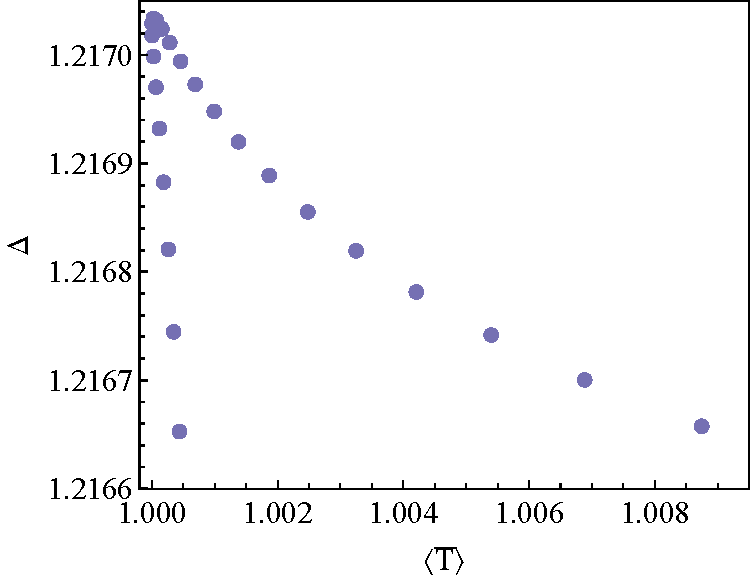
\includegraphics[width=3.0in]{gap-v-trace-delta.pdf}
\caption{\label{gap-v-trace-delta-plot}Many-body gap of $N_p=8$ interacting fermions at $\nu=1/3$ filling in the lowest band of the quartic model (\ref{quartic-harper}). In this plot, $\phi/\phi_0=1/24$, and the fermions interact via a repulsive next-nearest-neighbor potential. Each point correspond to a different value of $t_2$. This plot shows two different regimes with different dependence $\Delta$ on $\expval{T}$. The more slowly decreasing branch of the plot corresponds to $t_2 > -0.09$, and the other branch to $t_2 < -0.09$. The largest gap is observed where the two branches converge, at $t_2 = -0.09$.}
\end{figure}

\section{Spatially-inhomogeneous EM Response}
The perturbative response of QH fluids to static, spatially homogeneous electric fields is a key phenomenological feature of such fluids. This response is measured by the conductivity tensor $\sigma$ relating the electric current density $\mathbf{J}$ and perturbative electric field $\mathbf{E}$,
\begin{align}
\label{conductivity-eq}
J_{a} = \sigma_{ab}E_b.
\end{align}
In particular, one is interested in the transverse, or Hall, conductivity $\sigma_{xy}$, which takes the universal value
\begin{align*}
\sigma_{xy} = \sigma^{H} = \frac{\nu e^2}{2\pi \hbar}
\end{align*}
in quantum Hall fluids at filling fractional $\nu$.

Recent work has show that the perturbative response to spatially \textit{inhomogeneous} electric fields also encodes a universal phemonological feature of QH fluids, the Hall viscosity. The universal contribution to the Hall viscosity in a QH fluid on a surface with zero scalar curvature is\cite{Read2009}
\begin{align*}
\eta^H = \frac{1}{2}\hbar\bar{s}\rho_0,
\end{align*}
where $\rho_0$ is the mean density and $\bar{s}$ is the mean orbital angular momentum or topological spin of the fluid. For a Laughlin fluid with $\nu = \frac{1}{2k+1}$
\begin{align*}
\bar{s} = k + \frac{1}{2}
\end{align*}

If we consider the finite-wavevector version of (\ref{conductivity-eq}) above
\begin{align*}
J_{a}(\mathbf{q}) = \sigma_{ab}(\mathbf{q})E_b(\mathbf{q}),
\end{align*}
then the transverse conductivity is
\begin{align*}
\frac{\sigma_{xy}(\mathbf{q})}{\sigma^{H}} = 1 + (q\ell)^2\left(\frac{\eta^H}{\hbar \rho_0} - \frac{B^2}{2\nu u_{0}}\pdv[2]{u}{B}\right).
\end{align*}
Where $u(B)$ is the energy density as a function of magnetic field, and $u_0$ is the LLL energy density 
\begin{align*}
u_{0} = \frac{\hbar\omega/2}{2\pi\ell^2}.
\end{align*}

Ref. \onlinecite{em_response} presents a derivation of two transverse current responses in Chern bands to an applied inhomogeneous electric field. The first is the current per state or current per orbital, which is the current response of a single filled state within a Chern bands.
\begin{align}
\label{current-per-orbital}
\expval{I_{yn}} = -i\sum_{m\neq n} \mel{n,k}{\comm{y}{H}}{m,k}\frac{\mel{m,k}{V(x)}{n,k}}{E_n-E_m} + \text{h.c.}
\end{align}
The second response is the real-space current density, 
\begin{align}
\label{current-density}
J_{yn}(\mathbf{r}_0) = \sum_{k,m\neq n} \mel{n,k}{j_y(\mathbf{r}_0)}{m,k} \frac{\mel{m,k}{V(x)}{n,k}}{E_n-E_m} + \text{h.c.},
\end{align}
where $j_y(\mathbf{r}_0)$ is the symmetrized current density operator
\begin{align*}
j_y(\mathbf{r}_0) = \frac{1}{2}\left(I_y \delta(\mathbf{r} - \mathbf{r}_0) + \delta(\mathbf{r} - \mathbf{r}_0)I_y \right).
\end{align*}
This expression for $J_{yn}(\mathbf{r}_0)$ is equivalent to that obtained by a linear response calculation. The factor of $H$ in the current per orbital cancels the energy demoniator, so that $\expval{I_y}_{n,k}$ depends only on the band projectors and not on the energy dispersion. In contrast, this cancellation does not occur in the case of the current density. For a generic potential $V(x)$, we can write
\begin{align*}
V(x) = \sum c_p (x - x_0)^p,
\end{align*}
and in terms of the expansion coefficients 
\begin{align*}
\end{align*}

In the case of non-Landau level models, the above expressions (\ref{current-per-orbital}) and (\ref{current-density}) still hold, with the caveats that we must calculate the current operator using the non-Landau hamiltonian and interpret the states $\ket{n,k}$ as eigenstates of this hamiltonian. We have seen that we can obtain these perturbative eigenstates numerically by considering a finite-dimensional truncation of the hamiltonian written in the Landau level basis. In this way, we can numerically calculate these current responses for the case of our non-Landau bands. This calculation is carried out in detail for the $C_4$ symmetric models in Ref. [...].


\section{Conclusion}
In conclusion, we have constructed a Harper-Hofstadter model with cyclotron orbits that are distinct from Landau levels in the continuum limit. This provides a regime in which to study the quantum Hall effect that is distinct from both the Landau level 2DEG and FCI models. 

While we have focused on a particular choice of hopping amplitudes, by including longer-range hoppings and tuning them appropriately, one may obtain arbitrary inversion-symmetric dispersion relations. In particular, we could arrage our hamiltonian so that both quadratic and quartic terms vanish, leaving only a sextic term -- and so on. Put slightly differently, the construction that we have outlined here may in principle be used to construct infinite families of lattice hamiltonians that do not have Landau levels as their continuum cyclotron orbits.

One drawback of our numerical approach is that we diagonalize the many-body interaction hamiltonian on a lattice. While this is not a problem in the FCI regime, it may obscure the physics in the continuum regime, for example by gapping potential symmetry-breaking Goldstone modes that would be gapless in the continuum. Using DMRG or other numerical techniques that do not rely directly on a tight-binding description may rememedy this. Another drawback of constructing continuum bands from lattice model is that the continuum models inherit non-generic point-group symmetries from the lattice geometry, so that we do not obtain fully generic bands in this way.

\begin{acknowledgments}
The authors thank Tom Jackson for collaboration on related work and for his band geometry code. We also thank authors of the DiagHam package, which was used in this work.

\end{acknowledgments}
\bibliographystyle{apsrev4-1}
\bibliography{landau-orbits}
%\bibliography{quartic-zotero/quartic-zotero}

\clearpage
\appendix
\section{Weak-field effective hamiltonian for Hofstadter model $C_4$ symmetric NNN hopping}
For completeness, we reproduce here the  Hofstadter model with all next-nearest-neighbor (NNN) hopping terms that respect $C_4$ symmetry, including the hopping diagonally across a plaquette. The tight-binding hamiltonian is
\begin{align*}
H_0 = &-t_1 \left(T_x + T_y\right)\nonumber - t_2 \left(T_x^{2} + T_y^{2}\right)\\ &- t_3 \left(T_xT_y + T_y T_x\right) + \text{h.c.}
\end{align*}

We can write this in terms of the generators $K_a$ as
\begin{align*}
H_0 = &-2t_1 \left[\cos\left(K_x\right) + \cos\left(K_y\right)\right]\\ &-2t_2 \left[\cos\left(2K_x\right)+\cos\left(2K_y\right)\right]\\ &- 4t_3 \cosh\left(\frac{\epsilon^2}{2}\right)\cos\left(K_x + K_y\right).
\end{align*}
The factor of $\cosh(\epsilon^2/2)$ is non-universal and results from our ordering prescription.

Expanding to quartic order, we obtain the low-$\epsilon$ effective hamiltonian
\begin{align*}
H_{\text{eff}} = h_{ab}K_a K_b + \lambda_{abcd} K_a K_b K_c K_d 
\end{align*}

with coefficients

\begin{align*}
h_{11} = h_{22} &= t_1 + 4t_2 + 2t_3,\\
h_{12} &= 2t_3,
\end{align*}
and 
% \begin{align*}
% \lambda_{1111} &= \lambda_{2222} = -\frac{1}{3}\left(t_1/4 + 4t_2 + t_3/2\right)
% \lambda_{1112}  &= \lambda_{1222} = -t_3/3\\
% \lambda_{1122} &= -t_3/2
% \begin{align*}
\begin{align*}
\lambda_{1111} = \lambda_{2222} &= -\frac{1}{3}\left(\frac{t_1}{4} + 4t_2 + \frac{t_3}{2} \right),\\
\lambda_{1112}  = \lambda_{1222} &= -t_3/3,\\
\lambda_{1122} &= -t_3/2.
\end{align*}

% \section{Translation operators and magnetic unit cell}
% We will assume that the hopping amplitude between any two sites on the lattice is generically non-zero. We index the sites of the lattice by a vector $\mathbf{m} = (m_1, m_2)$ with integer components. Let $c^{\dag}_{\mathbf{m}}$ ($c_{\mathbf{m}}$) create (annihilate) an electron at site $\mathbf{m}$ of the lattice. We have the usual fermion anticommutation relations $\left\{c_{\mathbf{m}},c_{\mathbf{n}}^{\dag}\right\} = \delta_{\mathbf{m} \mathbf{n}}$. The single-particle Hilbert space is spanned by the space of states $\ket{\mathbf{m}}$ with the electron occupying site $\mathbf{m}$. The hamiltonian in this representation is
% \begin{align*}
% H_0 &= -\sum_{\mathbf{m}\neq \mathbf{n}}\left( t_{\mathbf{m}\mathbf{n}} c^{\dag}_\mathbf{n} c_\mathbf{m}  + t_{\mathbf{n}\mathbf{m}} c^{\dag}_{\mathbf{m}} c_{\mathbf{n}}\right).\\
% \end{align*}
% Note that we are excluding onsite/mass terms from the above hamiltonian; this is because a translation-invariant mass term simply shifts $H$ by a constant. We define lattice translation operators $T_a = \sum_{\bfm} c^{\dag}_{\mathbf{m} + \mathbf{e}_a}c_{\mathbf{m}}$, where $e_1=(1,0)$, $e_2=(0,1)$. We can write the hamiltonian in terms of these as
% \begin{align}
% \label{eq-b0-lattice-hamiltonian}
% H_0 = -\sum_{j,k} t_{jk} \left(T_x^j T_y^k + (T^{\dag}_2)^{k} (T^{\dag}_1)^{j}\right)
% \end{align}
% We stipulate that this hamiltonian should be time-reversal invariant in the absence of any magnetic flux, so the $t_{jk}$ will be real here and in the following.

% In the LL problem, guiding-center translations commute with the hamiltonian and generate the space of perfectly degenerate states within a single Landau level. In the lattice case, we have discrete rather than continuous translation symmetry, and the translation operators that commute with the hamiltonian are the \textit{magnetic translation operators} $\widetilde{U}_a$, which take the same form as the $T_a$:
% \begin{align*}
% \widetilde{U}_a = \sum_{\mathbf{m}} e^{i\chi_a(\mathbf{m})} c^{\dag}_{\mathbf{m} + \mathbf{e}_a}c_{\mathbf{m}}.
% \end{align*}
% In order for the lattice and magnetic translations to commute, the guiding-center gauge fluxes $\chi_a$ must satisfy
% \begin{align*}
% \Delta_a \theta_b = \Delta_b\chi_a,
% \end{align*}
% which implies
% \begin{align*}
% \Delta_1\chi_2 - \Delta_2 \chi_1 = -\varepsilon^2.
% \end{align*}
% The minus sign on the right-hand sign shows that lattice translations $T_a$ and guiding-center translations $\widetilde{U}_a$ carry opposite handedness, in analogy with the opposite handedness implied by the commutators $\comm{R_a}{R_b} = i\ell^2 \epsilon_{ab}$ and $\comm{\mathcal{R}_a}{\mathcal{R}_b} = -i\ell^2 \epsilon_{ab}$ of the Landau level problem.

% Unlike in the continuum LL case, we can find operators that commute with $H_0$ and also with one another. To do so, we define a \textit{magnetic unit cell} (MUC) containing $m \times n$ lattice sites, where $m$ and $n$ are chosen such that the MUC contains an integer number of flux quanta. Magnetic translations by one MUC commute, i.e. $\widetilde{U}_1^{m_1}\widetilde{U}_2^{m_2} = \widetilde{U}_2^{m_2}\widetilde{U}_1^{m_1}$. Since $\widetilde{U}_1$ and $\widetilde{U}_2$ commute with the hamiltonian, we can define their common eigenstates. This gives a ``guiding-center lattice'' of magnetic unit cells, each of which carries an internal Hilbert space corresponding to the cyclotron degrees of freedom.

% Since the MUC translation commute, we may define their simultaneous eigenstates
% \begin{align*}
% \widetilde{U}_1^{m_1}\ket{\mathbf{k}}&=e^{im_1 k_1}\ket{\mathbf{k}},\\
% \widetilde{U}_2^{m_2}\ket{\mathbf{k}}&=e^{im_2 k_2}\ket{\mathbf{k}},\\
% \end{align*}
% which serve as a basis for the guiding-center Hilbert space. The Bloch momentum $\mathbf{k}$ takes values in the \textit{magnetic Brillouin zone} (MBZ),
% \begin{align*}
% \text{MBZ} = \left\{\mathbf{k}\in\mathbf{R}^2, 0<k_1<\frac{2\pi}{m_1},0<k_2<\frac{2\pi}{m_2}\right\}.
% \end{align*}
% That is, the area of the MBZ is smaller than the physical BZ by a factor of $1/\epsilon^2$, reflecting the fact that we cannot simultaneously probe \textit{both} components of the momentum at smaller length scales.

% In the continuum LL problem, the choice of how to decompose the coordinates into Landau orbit and guiding center terms is a gauge choice, and cannot affect any observables. In the same way, the choice of how to decompose our lattice into a guiding-center lattice of MUCs does not affect any physics, so long as the MUCs enclose the same number of flux quanta.

\section{Zero-energy states for $a^4 + a^{\dag 4}$ hamiltonian}
\label{zero-enegy-quartic}
\begin{align*}
H = 
\end{align*}

% \section{Additional plots of many-body gaps}
% \begin{figure*}[thb]
% \centering
% 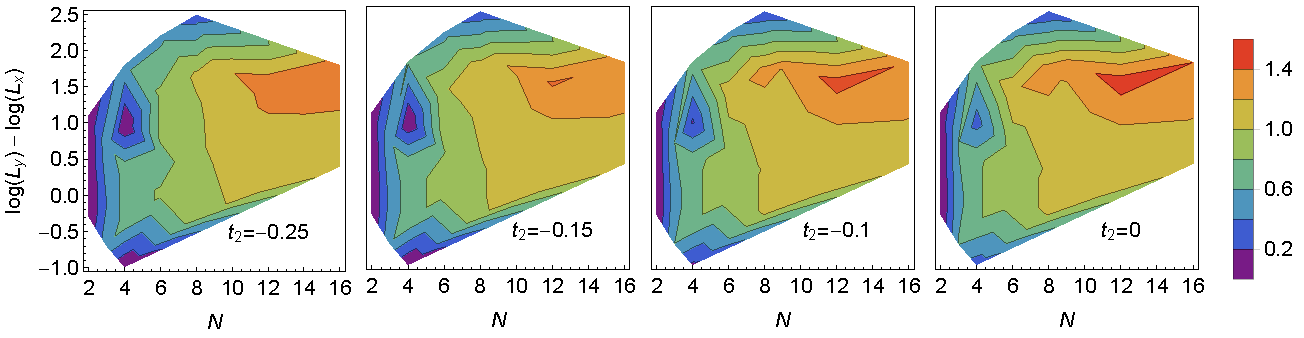
\includegraphics[width=6.3in]{gap-grid-2.pdf}
% \caption{Many-body gap of a $\nu=1/3$ Laughlin state of $N_p=8$ fermions in the lowest band of the modified Hofstadter model for $\phi = \phi_0/N$ and multiple values of $t_2$. The horizontal axis in each plot is the reciprocal $N$ of the flux per plaquette, while the vertical axis $\log(L_y/L_x)$ measures the overall anisotropy of the system with $L_x$ ($L_y$) the total number of lattice sites in the $x$ ($y$) direction. When $\log(L_y/L_x)=0$, the system is perfectly isotropic. }
% \end{figure*}

% \section{WKB treatment of Harper equation and generalizations}
% \label{wkb-appendix}
% For conceptual and notational clarity, we treat the case $\phi = 1/N$. The case $\phi=M/N$ is not essentially different, and details for the Hofstadter model in this case may be found in Ref. \onlinecite{Watson:1991gy}. We can recast the Harper equation for $k=0$ in terms of a continuous position $x=\phi n$
% \begin{align}
% \label{wkb-harper-eqn}
% \psi(x + \phi) + \psi(x - \phi) + 2 \cos(2\pi x)\psi(x) = - \epsilon \psi(x)
% \end{align}
% By making the WKB ansatz
% \begin{align}
% \label{wkb-ansatz}
% \psi(x) = \exp\left[\frac{1}{\phi}\left(S_0(x) + \phi S_1(x)\right)\right],
% \end{align}
% one obtains WKB solutions in the classically-forbidden region
% \begin{align*}
% \psi_{\text{exp}}^{\pm} = \frac{1}{\sqrt{\sinh q(x)}}\exp\left(\pm N \int^x ds\,q(s)\right)
% \end{align*}
% where 
% \begin{align*}
% q(x) = \cosh^{-1}\left[-\frac{\epsilon}{2} - 2\cos(2\pi x)\right].
% \end{align*}
% The exponential flatness of the dispersion in the energy, Berry curvature and Fubini-Study metric all follow from this tunneling wavefunction.

% In the case of the quartic and other higher-order models, the Landau-gauge Harper equation contains higher-order finite differences and additional periodic potential terms. For example, the Harper-type equation for the second-order model with $t_2/t_1 = \tau$ is
% \begin{align*}
% & \psi(x + \phi) + \psi(x - \phi) + \tau\left[\psi(x + 2\phi) + \psi(x - 2\phi)\right] \\ &= \left[-\epsilon - 2\cos(2\pi x) - 2\tau\cos(4\pi x)\right]\psi(x)
% \end{align*}
% More generally, for straight-line hopping models, we have
% \begin{align*}
% \sum_{n}\phi^{2n}\Delta^{(2n)}\psi(x) = \left[-\epsilon - V(x)\right]\psi(x).
% \end{align*}
% Since we are only interested in the leading-order exponential behavior, we may use a WKB ansatz of the same form (\ref{wkb-ansatz}) as in the second-order case, with the same conditions on the range of validity \cite{bender}.



% \begin{align*}
% \phi S_2(x) \ll 1
% \end{align*}
% \begin{align*}
% \frac{\psi(x) - \exp\left[\frac{1}{\phi}\left(S_0(x) + \phi S_1(x)\right)\right]}{\psi(x)} \sim \phi S_2(x)
% \end{align*}

\end{document}


